\documentclass[twoside]{book}

% Packages required by doxygen
\usepackage{fixltx2e}
\usepackage{calc}
\usepackage{doxygen}
\usepackage[export]{adjustbox} % also loads graphicx
\usepackage{graphicx}
\usepackage[utf8]{inputenc}
\usepackage{makeidx}
\usepackage{multicol}
\usepackage{multirow}
\PassOptionsToPackage{warn}{textcomp}
\usepackage{textcomp}
\usepackage[nointegrals]{wasysym}
\usepackage[table]{xcolor}

% Font selection
\usepackage[T1]{fontenc}
\usepackage[scaled=.90]{helvet}
\usepackage{courier}
\usepackage{amssymb}
\usepackage{sectsty}
\renewcommand{\familydefault}{\sfdefault}
\allsectionsfont{%
  \fontseries{bc}\selectfont%
  \color{darkgray}%
}
\renewcommand{\DoxyLabelFont}{%
  \fontseries{bc}\selectfont%
  \color{darkgray}%
}
\newcommand{\+}{\discretionary{\mbox{\scriptsize$\hookleftarrow$}}{}{}}

% Page & text layout
\usepackage{geometry}
\geometry{%
  a4paper,%
  top=2.5cm,%
  bottom=2.5cm,%
  left=2.5cm,%
  right=2.5cm%
}
\tolerance=750
\hfuzz=15pt
\hbadness=750
\setlength{\emergencystretch}{15pt}
\setlength{\parindent}{0cm}
\setlength{\parskip}{0.2cm}
\makeatletter
\renewcommand{\paragraph}{%
  \@startsection{paragraph}{4}{0ex}{-1.0ex}{1.0ex}{%
    \normalfont\normalsize\bfseries\SS@parafont%
  }%
}
\renewcommand{\subparagraph}{%
  \@startsection{subparagraph}{5}{0ex}{-1.0ex}{1.0ex}{%
    \normalfont\normalsize\bfseries\SS@subparafont%
  }%
}
\makeatother

% Headers & footers
\usepackage{fancyhdr}
\pagestyle{fancyplain}
\fancyhead[LE]{\fancyplain{}{\bfseries\thepage}}
\fancyhead[CE]{\fancyplain{}{}}
\fancyhead[RE]{\fancyplain{}{\bfseries\leftmark}}
\fancyhead[LO]{\fancyplain{}{\bfseries\rightmark}}
\fancyhead[CO]{\fancyplain{}{}}
\fancyhead[RO]{\fancyplain{}{\bfseries\thepage}}
\fancyfoot[LE]{\fancyplain{}{}}
\fancyfoot[CE]{\fancyplain{}{}}
\fancyfoot[RE]{\fancyplain{}{\bfseries\scriptsize Generated on Mon Dec 19 2016 05\+:51\+:07 for Unicode by Doxygen }}
\fancyfoot[LO]{\fancyplain{}{\bfseries\scriptsize Generated on Mon Dec 19 2016 05\+:51\+:07 for Unicode by Doxygen }}
\fancyfoot[CO]{\fancyplain{}{}}
\fancyfoot[RO]{\fancyplain{}{}}
\renewcommand{\footrulewidth}{0.4pt}
\renewcommand{\chaptermark}[1]{%
  \markboth{#1}{}%
}
\renewcommand{\sectionmark}[1]{%
  \markright{\thesection\ #1}%
}

% Indices & bibliography
\usepackage{natbib}
\usepackage[titles]{tocloft}
\setcounter{tocdepth}{3}
\setcounter{secnumdepth}{5}
\makeindex

% Hyperlinks (required, but should be loaded last)
\usepackage{ifpdf}
\ifpdf
  \usepackage[pdftex,pagebackref=true]{hyperref}
\else
  \usepackage[ps2pdf,pagebackref=true]{hyperref}
\fi
\hypersetup{%
  colorlinks=true,%
  linkcolor=blue,%
  citecolor=blue,%
  unicode%
}

% Custom commands
\newcommand{\clearemptydoublepage}{%
  \newpage{\pagestyle{empty}\cleardoublepage}%
}


%===== C O N T E N T S =====

\begin{document}

% Titlepage & ToC
\hypersetup{pageanchor=false,
             bookmarks=true,
             bookmarksnumbered=true,
             pdfencoding=unicode
            }
\pagenumbering{roman}
\begin{titlepage}
\vspace*{7cm}
\begin{center}%
{\Large Unicode }\\
\vspace*{1cm}
{\large Generated by Doxygen 1.8.10}\\
\vspace*{0.5cm}
{\small Mon Dec 19 2016 05:51:07}\\
\end{center}
\end{titlepage}
\clearemptydoublepage
\tableofcontents
\clearemptydoublepage
\pagenumbering{arabic}
\hypersetup{pageanchor=true}

%--- Begin generated contents ---
\chapter{Unicode dynamic lib for scripting language support of high speed lexing}
\label{md__r_e_a_d_m_e}
\hypertarget{md__r_e_a_d_m_e}{}
This library contains modules for efficient lexical operations on Unicode strings to support simple generation of D\+S\+L (Domain Specific Languages).


\begin{DoxyCode}
1 Node.cpp is an O(1) dictionary for translating Codepoints to Tablenumbers.
2 Tree.cpp is an O(N) dictionary for translating u32strings to Canonical Lists.
\end{DoxyCode}


\subsection*{Requirements\+:}


\begin{DoxyItemize}
\item g++ (gnu c++ compiler) supporting the -\/std=c++11 flag
\item cpplint
\item valgrind
\item doxygen
\end{DoxyItemize}

\subsection*{Build\+:}


\begin{DoxyItemize}
\item make clean; clear; make
\end{DoxyItemize}

\subsection*{Theory\+:}

Dictionary lookup typically incurs a cost of calculating the hash followed by disambiguating the hash bucket. Both of these calculations can be expensive. The cost is fixed for hash tables with no collisions.

\hyperlink{class_node}{Node} and \hyperlink{class_tree}{Tree} are alternative algorithms for guaranteeing low fixed cost dictionary operations on simple Unicode codepoints (\hyperlink{class_node}{Node}) and simple Unicode codepoint strings (\hyperlink{class_tree}{Tree}).

\subsubsection*{Observations supporting the \hyperlink{class_node}{Node} implementation\+:}

Codepoints have 21 significant bits. Observe letter B converted to indices. 
\begin{DoxyCode}
1 B
2 0042                          hexadecimal
3 000000000000001000010         binary
4 000 000 000 000 001 000 010   7 groups of 3
5 a=0 b=0 c=0 d=0 e=1 f=0 g=2   position labels and indices
\end{DoxyCode}


Lookup is performed by multiple table dereferences to get new indices. The code for getting an association for a codepoint is\+: 
\begin{DoxyCode}
1 ((codepoint>>(n*3))&0xf) where a uses n==0, b uses n==1, etc...
2 lookup(codepoint) \{ return T[T[T[T[T[T[T[1][g]][f]][e]][d]][c]][b]][a] \}
\end{DoxyCode}

\begin{DoxyItemize}
\item 7 multiplies \# Can be eliminated by manifest constants
\item 7 shifts
\item 7 masks
\item 8 table dereferences
\item 29 total machine code operations in original i\+A\+P\+X86 8088 instructions
\item operation count may be less for more recent processors
\item memory consumption per layer is 32 bytes
\end{DoxyItemize}

Consider all the values to be hexadecimal. The initial table index is 1 because index 0 is used to flag errors. Suppose we want to associate the codepoint for letter \textquotesingle{}B\textquotesingle{} with its codepoint. In other words, this lookup will be the identity function lookup(42) = 42. We will restrict the hex representation to 16 bits for visual ease. Keep in mind that the full width is 21. We start by building a table T with the following contents\+: 
\begin{DoxyCode}
1 B
2 0042
3 000000000000001000011
4 000 000 000 000 001 000 010
5 a=0 b=0 c=0 d=0 e=1 f=0 g=2
6 T = [
7  [0000 0000 0000 0000 0000 0000 0000 0000]  # <- error layer (all zeros always)
8  [0002 0000 0000 0000 0000 0000 0000 0000]  # <- starting index for lookup
9  [0003 0000 0000 0000 0000 0000 0000 0000]
10  [0004 0000 0000 0000 0000 0000 0000 0000]
11  [0005 0000 0000 0000 0000 0000 0000 0000]
12  [0000 0006 0000 0000 0000 0000 0000 0000]
13  [0007 0000 0000 0000 0000 0000 0000 0000]
14  [0000 0000 0042 0000 0000 0000 0000 0000]  # <- layer containing association
15 ]
\end{DoxyCode}


Illustration of sequential dereferencing. 
\begin{DoxyCode}
1 T[1][a] yields 2 then
2 T[2][b] yields 3 then
3 T[3][c] yields 4 then
4 T[4][d] yields 5 then
5 T[5][e] yields 6 then
6 T[6][f] yields 7 then
7 T[7][g] yields 42  # The association
\end{DoxyCode}


If we want to add an association for \textquotesingle{}C\textquotesingle{} the table will look like this\+: 
\begin{DoxyCode}
1 C
2 0043
3 000000000000001000011
4 000 000 000 000 001 000 011
5 a=0 b=0 c=0 d=0 e=1 f=0 g=3
6 T = [
7  [0000 0000 0000 0000 0000 0000 0000 0000]
8  [0002 0000 0000 0000 0000 0000 0000 0000]
9  [0003 0000 0000 0000 0000 0000 0000 0000]
10  [0004 0000 0000 0000 0000 0000 0000 0000]
11  [0005 0000 0000 0000 0000 0000 0000 0000]
12  [0000 0006 0000 0000 0000 0000 0000 0000]
13  [0007 0000 0000 0000 0000 0000 0000 0000]
14  [0000 0000 0042 0043 0000 0000 0000 0000] # <- table 8 has 0043 at offset 3
15 ]
\end{DoxyCode}
 Note how no layers were added to support \textquotesingle{}C\textquotesingle{}.

If we want to add an association for \textquotesingle{}L\textquotesingle{} the table will look like this. 
\begin{DoxyCode}
1 L
2 004C
3 000000000000001001100
4 000 000 000 000 001 001 100
5 a=0 b=0 c=0 d=0 e=1 f=1 g=4
6 T = [
7  [0000 0000 0000 0000 0000 0000 0000 0000]
8  [0002 0000 0000 0000 0000 0000 0000 0000]
9  [0003 0000 0000 0000 0000 0000 0000 0000]
10  [0004 0000 0000 0000 0000 0000 0000 0000]
11  [0005 0000 0000 0000 0000 0000 0000 0000]
12  [0000 0006 0000 0000 0000 0000 0000 0000]
13  [0007 0008 0000 0000 0000 0000 0000 0000] # <- see the addition of table 8
14  [0000 0000 0042 0043 0000 0000 0000 0000]
15  [0000 0000 0000 0000 004C 0000 0000 0000] # <- table 8 has 004C at offset 4
16 ]
\end{DoxyCode}


Now, let\textquotesingle{}s add the Chinese character for mountain U+5\+C71 
\begin{DoxyCode}
1 山
2 5C71
3 000000101110001110001 
4 000 000 101 110 001 110 001
5 a=0 b=0 c=5 d=6 e=1 f=6 g=1
6 T = [
7  [0000 0000 0000 0000 0000 0000 0000 0000]
8  [0002 0000 0000 0000 0000 0000 0000 0000]
9  [0003 0000 0000 0000 0000 0000 0000 0000]
10  [0004 0000 0000 0000 0000 0009 0000 0000] # <- see the addition of table 9
11  [0005 0000 0000 0000 0000 0000 0000 0000]
12  [0000 0006 0000 0000 0000 0000 0000 0000]
13  [0007 0008 0000 0000 0000 0000 0000 0000]
14  [0000 0000 0042 0043 0000 0000 0000 0000]
15  [0000 0000 0000 0000 004C 0000 0000 0000]
16  [0000 0000 0000 0000 0000 0000 000A 0000] # <- see the addition of table A
17  [0000 000B 0000 0000 0000 0000 0000 0000] # <- see the addition of table B
18  [0000 0000 0000 0000 0000 0000 000C 0000] # <- see the addition of table C
19  [0000 000D 0000 0000 0000 0000 0000 0000] # <- see the addition of table D
20  [0000 5C71 0000 0000 0000 0000 0000 0000] # <- table D has 5C71 at offset 1
21 ]
\end{DoxyCode}


Illustration of sequential dereferencing for that Chinese character. 
\begin{DoxyCode}
1 T[1][a] yields 2 then
2 T[2][b] yields 3 then
3 T[3][c] yields 9 then
4 T[4][d] yields A then
5 T[5][e] yields B then
6 T[6][f] yields C then
7 T[7][g] yields 5C71  # The association
\end{DoxyCode}


Using 3 groups of 7, the operation count drops to 17 and the memory consumption per layer is 512 bytes.

7 groups of 3 may look a bit inefficient with space, but 3 groups of 7 would be worse. The total consumed here by 7 groups of 3 is 14 $\ast$ 32 = 448 butes. For 3 groups of 7 this would be 6 $\ast$ 512 = 3017 bytes. 7 groups of 3 increases the calculation time by 7/3 or 2.\+3333... We choose to trade speed for space. These representations can be stored and recovered from disk.

Summary\+:
\begin{DoxyItemize}
\item Codepoints are intrinsically 21 bits.
\item 21 is the product 3 $\ast$ 7.
\item 3 groups of 7 bits or 7 groups of 3 bits will fit a codepoint perfectly.
\item a 32 bit internal codepoint or index occupies 4 bytes.
\item 3 bits supports 8 indices while 7 bits supports 128 indices.
\item 7 groups of 3 is used because the table layer size is small (32 bytes).
\item The initial association costs 8 $\ast$ 32 = 256 bytes.
\item Subsequent associations in-\/layer cost 0 additional bytes.
\item Subsequent associations out-\/of-\/layer cost at least one final layer each.
\item Worst case cost (i.\+e. 0x10\+F\+F\+F) costs 6 additional layers.
\end{DoxyItemize}

\subsection*{\hyperlink{class_node}{Node}\+: an O(1) state transition mechanism}

\hyperlink{class_node}{Node} acts as an O(1) dictionary to translate Unicode Codepoints or Unicode Codepoint classifications into table numbers. This enables rapid state machine operations.

\subsection*{\hyperlink{class_tree}{Tree}\+: an O(\+N) token lookup mechanism}

\hyperlink{class_tree}{Tree} acts as an O(\+N) dictionary to identify and/or canonicalize valid Unicode tokens. It can be used to recognize keywords. It can also be used to identify tokens that are absent from the dictionary. 
\chapter{Hierarchical Index}
\section{Class Hierarchy}
This inheritance list is sorted roughly, but not completely, alphabetically\+:\begin{DoxyCompactList}
\item dict\begin{DoxyCompactList}
\item \contentsline{section}{c.\+Dictionary.\+Dictionary}{\pageref{classc_1_1_dictionary_1_1_dictionary}}{}
\end{DoxyCompactList}
\item \contentsline{section}{Endian\+\_\+invariant32\+\_\+t}{\pageref{union_endian__invariant32__t}}{}
\item \contentsline{section}{entry\+\_\+t}{\pageref{structentry__t}}{}
\item object\begin{DoxyCompactList}
\item \contentsline{section}{c.\+Classify.\+Classify}{\pageref{classc_1_1_classify_1_1_classify}}{}
\item \contentsline{section}{c.\+De\+Brief.\+De\+Brief}{\pageref{classc_1_1_de_brief_1_1_de_brief}}{}
\item \contentsline{section}{c.\+De\+Brief.\+De\+Brief\+\_\+\+Module}{\pageref{classc_1_1_de_brief_1_1_de_brief___module}}{}
\item \contentsline{section}{c.\+Self.\+Self}{\pageref{classc_1_1_self_1_1_self}}{}
\end{DoxyCompactList}
\item \contentsline{section}{Omni}{\pageref{class_omni}}{}
\item \contentsline{section}{Page\+\_\+t}{\pageref{struct_page__t}}{}
\item \contentsline{section}{Page\+Spec\+\_\+t}{\pageref{struct_page_spec__t}}{}
\item De\+Brief\+\_\+\+Module\begin{DoxyCompactList}
\item \contentsline{section}{c.\+De\+Brief\+\_\+gcov.\+De\+Brief}{\pageref{classc_1_1_de_brief__gcov_1_1_de_brief}}{}
\item \contentsline{section}{c.\+De\+Brief\+\_\+out.\+De\+Brief}{\pageref{classc_1_1_de_brief__out_1_1_de_brief}}{}
\item \contentsline{section}{c.\+De\+Brief\+\_\+pep8.\+De\+Brief}{\pageref{classc_1_1_de_brief__pep8_1_1_de_brief}}{}
\item \contentsline{section}{c.\+De\+Brief\+\_\+pyflakes.\+De\+Brief}{\pageref{classc_1_1_de_brief__pyflakes_1_1_de_brief}}{}
\item \contentsline{section}{c.\+De\+Brief\+\_\+pylint.\+De\+Brief}{\pageref{classc_1_1_de_brief__pylint_1_1_de_brief}}{}
\item \contentsline{section}{c.\+De\+Brief\+\_\+valgrind.\+De\+Brief}{\pageref{classc_1_1_de_brief__valgrind_1_1_de_brief}}{}
\end{DoxyCompactList}
\end{DoxyCompactList}

\chapter{Class Index}
\section{Class List}
Here are the classes, structs, unions and interfaces with brief descriptions\+:\begin{DoxyCompactList}
\item\contentsline{section}{\hyperlink{classc_1_1_classify_1_1_classify}{c.\+Classify.\+Classify} }{\pageref{classc_1_1_classify_1_1_classify}}{}
\item\contentsline{section}{\hyperlink{union_endian__invariant32__t}{Endian\+\_\+invariant32\+\_\+t} }{\pageref{union_endian__invariant32__t}}{}
\item\contentsline{section}{\hyperlink{structentry__t}{entry\+\_\+t} }{\pageref{structentry__t}}{}
\item\contentsline{section}{\hyperlink{class_omni}{Omni} \\*Encoding/decoding algorithm (see en.\+wikipedia.\+org/wiki/\+Base64) }{\pageref{class_omni}}{}
\item\contentsline{section}{\hyperlink{classc_1_1_make_time_1_1_option}{c.\+Make\+Time.\+Option} }{\pageref{classc_1_1_make_time_1_1_option}}{}
\item\contentsline{section}{\hyperlink{classc_1_1_self_1_1_self}{c.\+Self.\+Self} }{\pageref{classc_1_1_self_1_1_self}}{}
\end{DoxyCompactList}

\chapter{Class Documentation}
\hypertarget{classc_1_1_classify_1_1_classify}{}\section{c.\+Classify.\+Classify Class Reference}
\label{classc_1_1_classify_1_1_classify}\index{c.\+Classify.\+Classify@{c.\+Classify.\+Classify}}
Inheritance diagram for c.\+Classify.\+Classify\+:\begin{figure}[H]
\begin{center}
\leavevmode
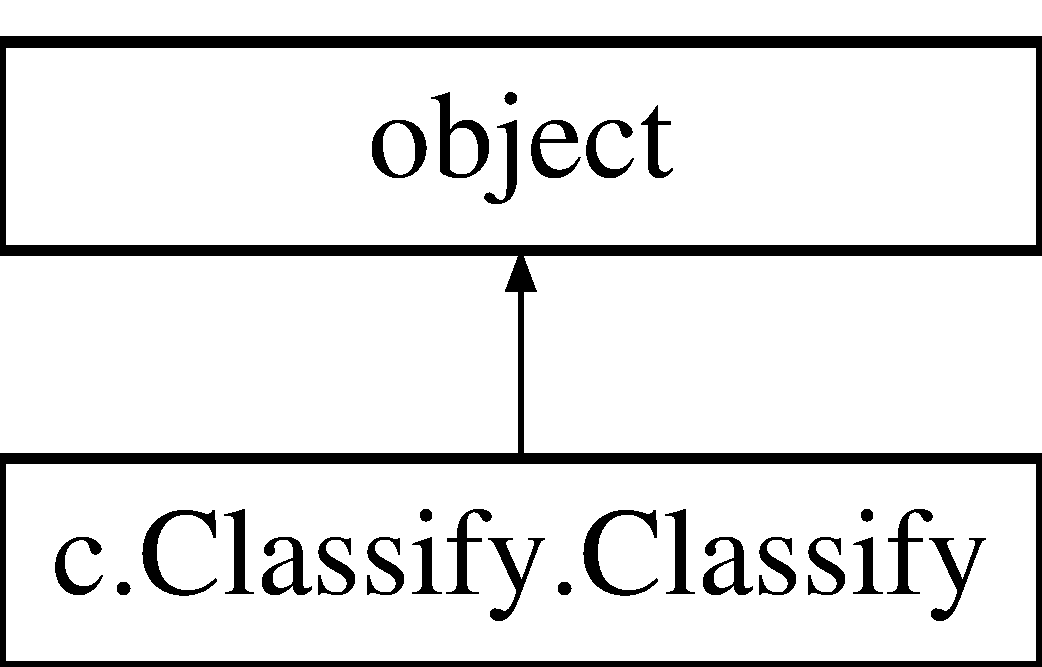
\includegraphics[height=2.000000cm]{classc_1_1_classify_1_1_classify}
\end{center}
\end{figure}
\subsection*{Public Member Functions}
\begin{DoxyCompactItemize}
\item 
def \hyperlink{classc_1_1_classify_1_1_classify_a398279537ff57bdd2d903fdfa2c398bf}{\+\_\+\+\_\+init\+\_\+\+\_\+} (self)
\item 
def \hyperlink{classc_1_1_classify_1_1_classify_a76c7951d7b300167925e145e58ed3fa3}{header} (self)
\item 
def \hyperlink{classc_1_1_classify_1_1_classify_a5d8e1a6fbcbab785107f9e3a40b7e154}{labels} (self)
\item 
def \hyperlink{classc_1_1_classify_1_1_classify_ace6a8a06833cfe31d3abcbce270817ad}{uniques} (self)
\item 
def \hyperlink{classc_1_1_classify_1_1_classify_a7c4ec3de2e18e3db3a03ddbca71ccba6}{indices} (self)
\item 
def \hyperlink{classc_1_1_classify_1_1_classify_ae0bfdd4ee16c94394efc666b4c501bcc}{classify} (self)
\item 
def \hyperlink{classc_1_1_classify_1_1_classify_ab723602c25ed262d0c38114d6f8da7bc}{constructor} (self)
\item 
\hypertarget{classc_1_1_classify_1_1_classify_a178781aedac62cb6da8ef6cd71071b12}{}def {\bfseries \+\_\+\+\_\+call\+\_\+\+\_\+} (self)\label{classc_1_1_classify_1_1_classify_a178781aedac62cb6da8ef6cd71071b12}

\item 
\hypertarget{classc_1_1_classify_1_1_classify_a45fb26bfae7f894804ed286cac33f379}{}def {\bfseries \+\_\+\+\_\+str\+\_\+\+\_\+} (self)\label{classc_1_1_classify_1_1_classify_a45fb26bfae7f894804ed286cac33f379}

\end{DoxyCompactItemize}
\subsection*{Public Attributes}
\begin{DoxyCompactItemize}
\item 
\hypertarget{classc_1_1_classify_1_1_classify_a39504bd936bf5576befb10e0ac43d83f}{}{\bfseries label}\label{classc_1_1_classify_1_1_classify_a39504bd936bf5576befb10e0ac43d83f}

\item 
\hypertarget{classc_1_1_classify_1_1_classify_a4f7fa627ce6c996d15b94b95fc308efd}{}{\bfseries index}\label{classc_1_1_classify_1_1_classify_a4f7fa627ce6c996d15b94b95fc308efd}

\item 
\hypertarget{classc_1_1_classify_1_1_classify_ae16c6fab346508b48b720cd04e9ce7df}{}{\bfseries fields}\label{classc_1_1_classify_1_1_classify_ae16c6fab346508b48b720cd04e9ce7df}

\item 
\hypertarget{classc_1_1_classify_1_1_classify_a1e4a9a02e19f108821677534f7e8d60a}{}{\bfseries ranges}\label{classc_1_1_classify_1_1_classify_a1e4a9a02e19f108821677534f7e8d60a}

\item 
\hypertarget{classc_1_1_classify_1_1_classify_afdb329410c16ea92a7ac17476f576fde}{}{\bfseries starts}\label{classc_1_1_classify_1_1_classify_afdb329410c16ea92a7ac17476f576fde}

\item 
\hypertarget{classc_1_1_classify_1_1_classify_a301a21d13817bbbbf07d6af1226c244a}{}{\bfseries text}\label{classc_1_1_classify_1_1_classify_a301a21d13817bbbbf07d6af1226c244a}

\item 
\hypertarget{classc_1_1_classify_1_1_classify_ab4f473fa1589075793de2f93ebe9bfa6}{}{\bfseries assoc}\label{classc_1_1_classify_1_1_classify_ab4f473fa1589075793de2f93ebe9bfa6}

\item 
\hypertarget{classc_1_1_classify_1_1_classify_ac670ebd238054400347771255ad5d043}{}{\bfseries pairs}\label{classc_1_1_classify_1_1_classify_ac670ebd238054400347771255ad5d043}

\end{DoxyCompactItemize}


\subsection{Detailed Description}
\begin{DoxyVerb}Generate Classify.c and Classify.h\end{DoxyVerb}
 

\subsection{Constructor \& Destructor Documentation}
\hypertarget{classc_1_1_classify_1_1_classify_a398279537ff57bdd2d903fdfa2c398bf}{}\index{c\+::\+Classify\+::\+Classify@{c\+::\+Classify\+::\+Classify}!\+\_\+\+\_\+init\+\_\+\+\_\+@{\+\_\+\+\_\+init\+\_\+\+\_\+}}
\index{\+\_\+\+\_\+init\+\_\+\+\_\+@{\+\_\+\+\_\+init\+\_\+\+\_\+}!c\+::\+Classify\+::\+Classify@{c\+::\+Classify\+::\+Classify}}
\subsubsection[{\+\_\+\+\_\+init\+\_\+\+\_\+(self)}]{\setlength{\rightskip}{0pt plus 5cm}def c.\+Classify.\+Classify.\+\_\+\+\_\+init\+\_\+\+\_\+ (
\begin{DoxyParamCaption}
\item[{}]{self}
\end{DoxyParamCaption}
)}\label{classc_1_1_classify_1_1_classify_a398279537ff57bdd2d903fdfa2c398bf}
\begin{DoxyVerb}This process may be slightly inefficient, but that is for clarity.
\end{DoxyVerb}
 

\subsection{Member Function Documentation}
\hypertarget{classc_1_1_classify_1_1_classify_ae0bfdd4ee16c94394efc666b4c501bcc}{}\index{c\+::\+Classify\+::\+Classify@{c\+::\+Classify\+::\+Classify}!classify@{classify}}
\index{classify@{classify}!c\+::\+Classify\+::\+Classify@{c\+::\+Classify\+::\+Classify}}
\subsubsection[{classify(self)}]{\setlength{\rightskip}{0pt plus 5cm}def c.\+Classify.\+Classify.\+classify (
\begin{DoxyParamCaption}
\item[{}]{self}
\end{DoxyParamCaption}
)}\label{classc_1_1_classify_1_1_classify_ae0bfdd4ee16c94394efc666b4c501bcc}
\begin{DoxyVerb}/**
 * Classify is the array of indices to classification labels for ALL codepoints
 */
unsigned char Classify[0x110000];
\end{DoxyVerb}
 \hypertarget{classc_1_1_classify_1_1_classify_ab723602c25ed262d0c38114d6f8da7bc}{}\index{c\+::\+Classify\+::\+Classify@{c\+::\+Classify\+::\+Classify}!constructor@{constructor}}
\index{constructor@{constructor}!c\+::\+Classify\+::\+Classify@{c\+::\+Classify\+::\+Classify}}
\subsubsection[{constructor(self)}]{\setlength{\rightskip}{0pt plus 5cm}def c.\+Classify.\+Classify.\+constructor (
\begin{DoxyParamCaption}
\item[{}]{self}
\end{DoxyParamCaption}
)}\label{classc_1_1_classify_1_1_classify_ab723602c25ed262d0c38114d6f8da7bc}
\begin{DoxyVerb}/**
 * Classify_init is run before main is called.
 * It initializes the Classify array from the RLE data.
 * https://www.hackerearth.com/practice/notes/
 *      functions-which-get-executed-before-and-after-main-in-c/
 * http://www.geeksforgeeks.org/
 *      functions-that-are-executed-before-and-after-main-in-c/
 */
__attribute__((constructor))
void Classify_init(void) {
    unsigned codepoint = 0;

    for (int i=0; i < 3655 ; ++i) {
const unsigned *pair = Classify_uniq[Classify_RLE[i]];
unsigned index = pair[0];
unsigned width = pair[1];

for (unsigned n=0; n < width; ++n)
    Classify[codepoint++] = (unsigned char)index;
    }
}
\end{DoxyVerb}
 \hypertarget{classc_1_1_classify_1_1_classify_a76c7951d7b300167925e145e58ed3fa3}{}\index{c\+::\+Classify\+::\+Classify@{c\+::\+Classify\+::\+Classify}!header@{header}}
\index{header@{header}!c\+::\+Classify\+::\+Classify@{c\+::\+Classify\+::\+Classify}}
\subsubsection[{header(self)}]{\setlength{\rightskip}{0pt plus 5cm}def c.\+Classify.\+Classify.\+header (
\begin{DoxyParamCaption}
\item[{}]{self}
\end{DoxyParamCaption}
)}\label{classc_1_1_classify_1_1_classify_a76c7951d7b300167925e145e58ed3fa3}
\begin{DoxyVerb}\
/* Classify.c Copyright(c) 2016 Jonathan D. Lettvin, All Rights Reserved. */

/** Classify.h and Classify.c
These files contain sufficient data to reconstruct the array "Classify"
containing the index to the string in "Classify_Label" for each codepoint.
The reason for the odd construction is that classifications are
highly concentrated into RunLengths.
Classify_uniq is an array of ALL uniq pairs of (index, length)
found when constructing the Classify array.
The odd-looking "Classigy_RLE" is the index into Classify_uniq
to a given pair.
The sequence of pairs fills the entire valid codepoint range with
index-to-label.
The classification of a codepoint devolves into the simple:
    Classify[codepoint];
which returns a NUL terminated label char*.

Immediately after the declaration of Classify is an
__attribute__((constructor)) which is executed before entry into main
for gnu c compilers.
This guarantees that Classify is filled and ready at runtime
after being reconstructed from RunLength pairs.
 */


#include "Classify.h"
\end{DoxyVerb}
 \hypertarget{classc_1_1_classify_1_1_classify_a7c4ec3de2e18e3db3a03ddbca71ccba6}{}\index{c\+::\+Classify\+::\+Classify@{c\+::\+Classify\+::\+Classify}!indices@{indices}}
\index{indices@{indices}!c\+::\+Classify\+::\+Classify@{c\+::\+Classify\+::\+Classify}}
\subsubsection[{indices(self)}]{\setlength{\rightskip}{0pt plus 5cm}def c.\+Classify.\+Classify.\+indices (
\begin{DoxyParamCaption}
\item[{}]{self}
\end{DoxyParamCaption}
)}\label{classc_1_1_classify_1_1_classify_a7c4ec3de2e18e3db3a03ddbca71ccba6}
\begin{DoxyVerb}/**
 * Classify_RLE contains indices to pairs in the Classify_uniq table.
 * The sequence of pairs is used to fill the Classify array.
 */
static const unsigned Classify_RLE[%d] = {
%s
};
\end{DoxyVerb}
 \hypertarget{classc_1_1_classify_1_1_classify_a5d8e1a6fbcbab785107f9e3a40b7e154}{}\index{c\+::\+Classify\+::\+Classify@{c\+::\+Classify\+::\+Classify}!labels@{labels}}
\index{labels@{labels}!c\+::\+Classify\+::\+Classify@{c\+::\+Classify\+::\+Classify}}
\subsubsection[{labels(self)}]{\setlength{\rightskip}{0pt plus 5cm}def c.\+Classify.\+Classify.\+labels (
\begin{DoxyParamCaption}
\item[{}]{self}
\end{DoxyParamCaption}
)}\label{classc_1_1_classify_1_1_classify_a5d8e1a6fbcbab785107f9e3a40b7e154}
\begin{DoxyVerb}/**
 * Classify_Label contains all legal top-level Unicode codepoint classifiers
 */
const char Classify_Label[%d][3] = {
%s
};
\end{DoxyVerb}
 \hypertarget{classc_1_1_classify_1_1_classify_ace6a8a06833cfe31d3abcbce270817ad}{}\index{c\+::\+Classify\+::\+Classify@{c\+::\+Classify\+::\+Classify}!uniques@{uniques}}
\index{uniques@{uniques}!c\+::\+Classify\+::\+Classify@{c\+::\+Classify\+::\+Classify}}
\subsubsection[{uniques(self)}]{\setlength{\rightskip}{0pt plus 5cm}def c.\+Classify.\+Classify.\+uniques (
\begin{DoxyParamCaption}
\item[{}]{self}
\end{DoxyParamCaption}
)}\label{classc_1_1_classify_1_1_classify_ace6a8a06833cfe31d3abcbce270817ad}
\begin{DoxyVerb}/**
 * Classify_uniq contains all unique (label_index, length) pairs.
 * This is useful because the actual pairs are quire repetitive.
 */
static const unsigned Classify_uniq[%d][2] = {
%s
};
\end{DoxyVerb}
 

The documentation for this class was generated from the following file\+:\begin{DoxyCompactItemize}
\item 
Classify.\+py\end{DoxyCompactItemize}

\hypertarget{union_endian__invariant32__t}{}\section{Endian\+\_\+invariant32\+\_\+t Union Reference}
\label{union_endian__invariant32__t}\index{Endian\+\_\+invariant32\+\_\+t@{Endian\+\_\+invariant32\+\_\+t}}
\subsection*{Public Attributes}
\begin{DoxyCompactItemize}
\item 
\hypertarget{union_endian__invariant32__t_a784127cdb901408682dac3f36808845a}{}ue2\+\_\+t \hyperlink{union_endian__invariant32__t_a784127cdb901408682dac3f36808845a}{u32}\label{union_endian__invariant32__t_a784127cdb901408682dac3f36808845a}

\begin{DoxyCompactList}\small\item\em data as a 32 bit representation \end{DoxyCompactList}\item 
\hypertarget{union_endian__invariant32__t_ada459fdec7e2170806c48997490870ad}{}ue0\+\_\+t \hyperlink{union_endian__invariant32__t_ada459fdec7e2170806c48997490870ad}{u8} \mbox{[}4\mbox{]}\label{union_endian__invariant32__t_ada459fdec7e2170806c48997490870ad}

\begin{DoxyCompactList}\small\item\em data as 4 8 bit representations \end{DoxyCompactList}\end{DoxyCompactItemize}


The documentation for this union was generated from the following file\+:\begin{DoxyCompactItemize}
\item 
Endian.\+h\end{DoxyCompactItemize}

\hypertarget{structentry__t}{}\section{entry\+\_\+t Struct Reference}
\label{structentry__t}\index{entry\+\_\+t@{entry\+\_\+t}}


{\ttfamily \#include $<$Unicode.\+h$>$}

\subsection*{Public Attributes}
\begin{DoxyCompactItemize}
\item 
\hypertarget{structentry__t_a1e82af966dbc9caa8129a7b4320417bc}{}codepoint\+\_\+t \hyperlink{structentry__t_a1e82af966dbc9caa8129a7b4320417bc}{codepoint}\label{structentry__t_a1e82af966dbc9caa8129a7b4320417bc}

\begin{DoxyCompactList}\small\item\em the value \end{DoxyCompactList}\item 
\hypertarget{structentry__t_aee9f08e356b624555bb6101ea4633f3a}{}target\+\_\+t \hyperlink{structentry__t_aee9f08e356b624555bb6101ea4633f3a}{table}\label{structentry__t_aee9f08e356b624555bb6101ea4633f3a}

\begin{DoxyCompactList}\small\item\em the linkage \end{DoxyCompactList}\end{DoxyCompactItemize}


\subsection{Detailed Description}
A type to support linkage. 

The documentation for this struct was generated from the following file\+:\begin{DoxyCompactItemize}
\item 
Unicode.\+h\end{DoxyCompactItemize}

\hypertarget{class_omni}{}\section{Omni Class Reference}
\label{class_omni}\index{Omni@{Omni}}


encoding/decoding algorithm (see en.\+wikipedia.\+org/wiki/\+Base64).  




{\ttfamily \#include $<$B64.\+h$>$}



\subsection{Detailed Description}
encoding/decoding algorithm (see en.\+wikipedia.\+org/wiki/\+Base64). 

Conversions between U\+T\+F8 and char32\+\_\+t.

Common header.

Unit test support function.

memory management scheme to support sparse memory use.

codepoint classifier (lexer generics)

\hyperlink{_b64_8h_source}{B64.\+h} and B64.\+c

\begin{DoxyAuthor}{Author}
Jonathan D. Lettvin \href{mailto:jlettvin@gmail.com}{\tt jlettvin@gmail.\+com}
\end{DoxyAuthor}
\begin{DoxyVersion}{Version}
0.\+0.\+1
\end{DoxyVersion}
\begin{DoxyDate}{Date}
2016/12/10 09\+:47
\end{DoxyDate}
license G\+P\+Lv3

\begin{DoxyCopyright}{Copyright}
Copyright(\+C) 2016 Jonathan D. Lettvin, All Rights Reserved"
\end{DoxyCopyright}
Using these examples from wikipedia, a two-\/way transform is shown. \char`\"{}\+M\char`\"{} $<$=$>$ \char`\"{}\+T\+Q==\char`\"{} \char`\"{}\+Ma\char`\"{} $<$=$>$ \char`\"{}\+T\+W\+E=\char`\"{} \char`\"{}\+Man\char`\"{} $<$=$>$ \char`\"{}\+T\+W\+Fu\char`\"{}

8 bits taken 3 at a time is equal to 6 bits taken 4 at a time. In other words, encoding expands by 4/3 and decoding shrinkgs by 3/4.

The original 8 bit bytes are sliced up 6 bits at a time and the 6 bits are encoded as common A\+S\+C\+I\+I to avoid encoding problems. The absence of high bits and control characters is historically valuable. The example below shows how 3 bytes is converted to 6 bit fields and how those fields are related to encoding letters.

Man M a n 01001101 01100001 01101110 010011 010110 000101 101110 19 22 5 46 T=\mbox{[}19\mbox{]} W=\mbox{[}22\mbox{]} F=\mbox{[} 5\mbox{]} u=\mbox{[}46\mbox{]} T\+W\+Fu

These are the declared interface functions.

\hyperlink{_classify_8h_source}{Classify.\+h} and Classify.\+c

rief codepoint classifier (lexer generics)

uthor Jonathan D. Lettvin \href{mailto:jlettvin@gmail.com}{\tt jlettvin@gmail.\+com}

ersion 0.\+0.\+1

\begin{DoxyDate}{Date}
2016/12/10 09\+:47
\end{DoxyDate}
license G\+P\+Lv3

\begin{DoxyCopyright}{Copyright}
Copyright(\+C) 2016 Jonathan D. Lettvin, All Rights Reserved"
\end{DoxyCopyright}
\hyperlink{_classify_8h_source}{Classify.\+h} and Classify.\+c

\begin{DoxyAuthor}{Author}
Jonathan D. Lettvin \href{mailto:jlettvin@gmail.com}{\tt jlettvin@gmail.\+com}
\end{DoxyAuthor}
\begin{DoxyVersion}{Version}
0.\+0.\+1
\end{DoxyVersion}
\begin{DoxyDate}{Date}
2016/12/10 09\+:47
\end{DoxyDate}
license G\+P\+Lv3

\begin{DoxyCopyright}{Copyright}
Copyright(\+C) 2016 Jonathan D. Lettvin, All Rights Reserved"
\end{DoxyCopyright}
\hyperlink{_endian_8h_source}{Endian.\+h} and Endian.\+c

\begin{DoxyAuthor}{Author}
Jonathan D. Lettvin \href{mailto:jlettvin@gmail.com}{\tt jlettvin@gmail.\+com}
\end{DoxyAuthor}
\begin{DoxyVersion}{Version}
0.\+0.\+1
\end{DoxyVersion}
\begin{DoxyDate}{Date}
2016/12/10 09\+:47
\end{DoxyDate}
license G\+P\+Lv3

\begin{DoxyCopyright}{Copyright}
Copyright(\+C) 2016 Jonathan D. Lettvin, All Rights Reserved"
\end{DoxyCopyright}
\hyperlink{_page_8h_source}{Page.\+h} and Page.\+c

\begin{DoxyAuthor}{Author}
Jonathan D. Lettvin \href{mailto:jlettvin@gmail.com}{\tt jlettvin@gmail.\+com}
\end{DoxyAuthor}
\begin{DoxyVersion}{Version}
0.\+0.\+1
\end{DoxyVersion}
\begin{DoxyDate}{Date}
2016/12/10 09\+:47
\end{DoxyDate}
license G\+P\+Lv3

\begin{DoxyCopyright}{Copyright}
Copyright(\+C) 2016 Jonathan D. Lettvin, All Rights Reserved"
\end{DoxyCopyright}
passfail

\begin{DoxyAuthor}{Author}
Jonathan D. Lettvin \href{mailto:jlettvin@gmail.com}{\tt jlettvin@gmail.\+com}
\end{DoxyAuthor}
\begin{DoxyVersion}{Version}
0.\+0.\+1
\end{DoxyVersion}
\begin{DoxyDate}{Date}
2016/12/10 09\+:47
\end{DoxyDate}
license G\+P\+Lv3

\begin{DoxyCopyright}{Copyright}
Copyright(\+C) 2016 Jonathan D. Lettvin, All Rights Reserved"
\end{DoxyCopyright}
\begin{DoxyAuthor}{Author}
Jonathan D. Lettvin \href{mailto:jlettvin@gmail.com}{\tt jlettvin@gmail.\+com}
\end{DoxyAuthor}
\begin{DoxyVersion}{Version}
0.\+0.\+1
\end{DoxyVersion}
\begin{DoxyDate}{Date}
2016/12/10 09\+:47
\end{DoxyDate}
license G\+P\+Lv3

\begin{DoxyCopyright}{Copyright}
Copyright(\+C) 2016 Jonathan D. Lettvin, All Rights Reserved"
\end{DoxyCopyright}
\begin{DoxyAuthor}{Author}
Jonathan D. Lettvin \href{mailto:jlettvin@gmail.com}{\tt jlettvin@gmail.\+com}
\end{DoxyAuthor}
\begin{DoxyVersion}{Version}
0.\+0.\+1
\end{DoxyVersion}
\begin{DoxyDate}{Date}
2016/11/29 09\+:47
\end{DoxyDate}
license G\+P\+Lv3

\begin{DoxyCopyright}{Copyright}
Copyright(\+C) 2016 Jonathan D. Lettvin, All Rights Reserved"
\end{DoxyCopyright}
B\+A\+C\+K\+G\+R\+O\+U\+N\+D\+: \href{http://lemire.me/blog/2012/06/20/do-not-waste-time-with-stl-vectors/}{\tt http\+://lemire.\+me/blog/2012/06/20/do-\/not-\/waste-\/time-\/with-\/stl-\/vectors/} 

The documentation for this class was generated from the following file\+:\begin{DoxyCompactItemize}
\item 
B64.\+h\end{DoxyCompactItemize}

\hypertarget{classc_1_1_make_time_1_1_option}{}\section{c.\+Make\+Time.\+Option Class Reference}
\label{classc_1_1_make_time_1_1_option}\index{c.\+Make\+Time.\+Option@{c.\+Make\+Time.\+Option}}
Inheritance diagram for c.\+Make\+Time.\+Option\+:\begin{figure}[H]
\begin{center}
\leavevmode
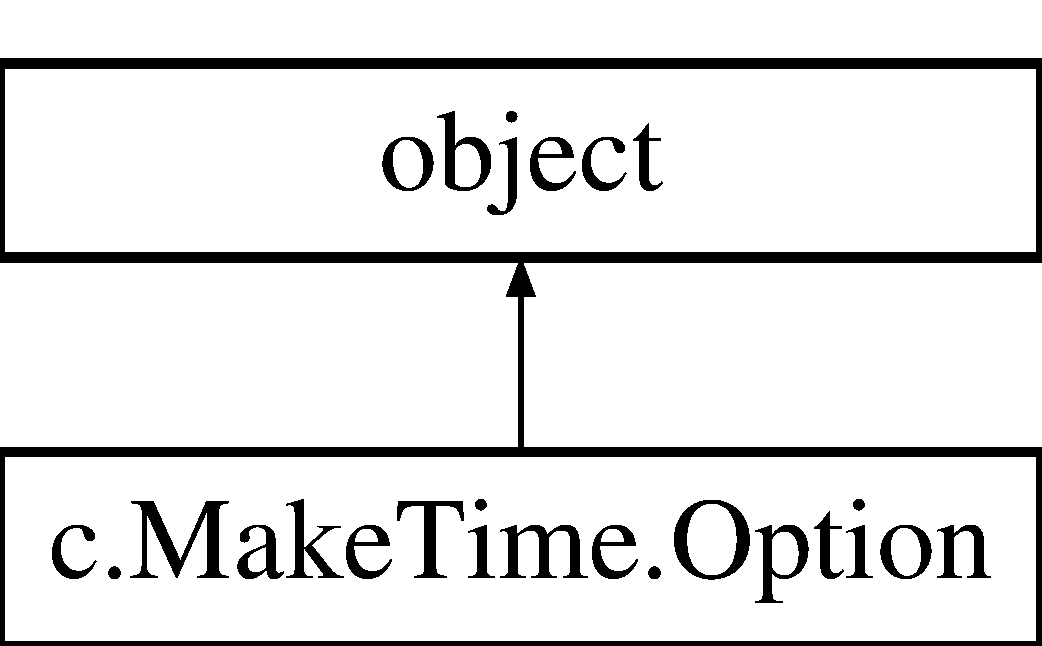
\includegraphics[height=2.000000cm]{classc_1_1_make_time_1_1_option}
\end{center}
\end{figure}
\subsection*{Static Public Member Functions}
\begin{DoxyCompactItemize}
\item 
\hypertarget{classc_1_1_make_time_1_1_option_ae180a2b27f60fa03d3666417bbdcda4e}{}def {\bfseries brief} (key)\label{classc_1_1_make_time_1_1_option_ae180a2b27f60fa03d3666417bbdcda4e}

\item 
\hypertarget{classc_1_1_make_time_1_1_option_ab5fd9c4360b6a6d6b3fba8257f144d50}{}def {\bfseries prose} (key)\label{classc_1_1_make_time_1_1_option_ab5fd9c4360b6a6d6b3fba8257f144d50}

\item 
\hypertarget{classc_1_1_make_time_1_1_option_a89e8b12beafc3c529b6c873f62339060}{}def {\bfseries help} (msg)\label{classc_1_1_make_time_1_1_option_a89e8b12beafc3c529b6c873f62339060}

\end{DoxyCompactItemize}
\subsection*{Static Public Attributes}
\begin{DoxyCompactItemize}
\item 
\hypertarget{classc_1_1_make_time_1_1_option_aeb22c8cafa69f0e4599c896ce54b4212}{}string {\bfseries store} = \char`\"{}Make\+Time.\+json\char`\"{}\label{classc_1_1_make_time_1_1_option_aeb22c8cafa69f0e4599c896ce54b4212}

\item 
\hypertarget{classc_1_1_make_time_1_1_option_a571699b044ea236a203ff2991b512684}{}dictionary {\bfseries key}\label{classc_1_1_make_time_1_1_option_a571699b044ea236a203ff2991b512684}

\item 
\hypertarget{classc_1_1_make_time_1_1_option_a25107ccb7b35e7df1a5e012c7ddf41de}{}list {\bfseries order} = \mbox{[}\textquotesingle{}clear\textquotesingle{}, \textquotesingle{}report\textquotesingle{}, \textquotesingle{}test\textquotesingle{}, \textquotesingle{}help\textquotesingle{}\mbox{]}\label{classc_1_1_make_time_1_1_option_a25107ccb7b35e7df1a5e012c7ddf41de}

\end{DoxyCompactItemize}


\subsection{Detailed Description}
\begin{DoxyVerb}The first argument to {COMMAND} must be either an option or a label.
This class handles all data and display related to options.
All viable options are keys in the dictionary.
Each option has a list of variants which may appear on the command-line.
This class is not intended to be instanced.
All operations use static members and methods.
\end{DoxyVerb}
 

The documentation for this class was generated from the following file\+:\begin{DoxyCompactItemize}
\item 
Make\+Time.\+py\end{DoxyCompactItemize}

\hypertarget{classc_1_1_self_1_1_self}{}\section{c.\+Self.\+Self Class Reference}
\label{classc_1_1_self_1_1_self}\index{c.\+Self.\+Self@{c.\+Self.\+Self}}
Inheritance diagram for c.\+Self.\+Self\+:\begin{figure}[H]
\begin{center}
\leavevmode
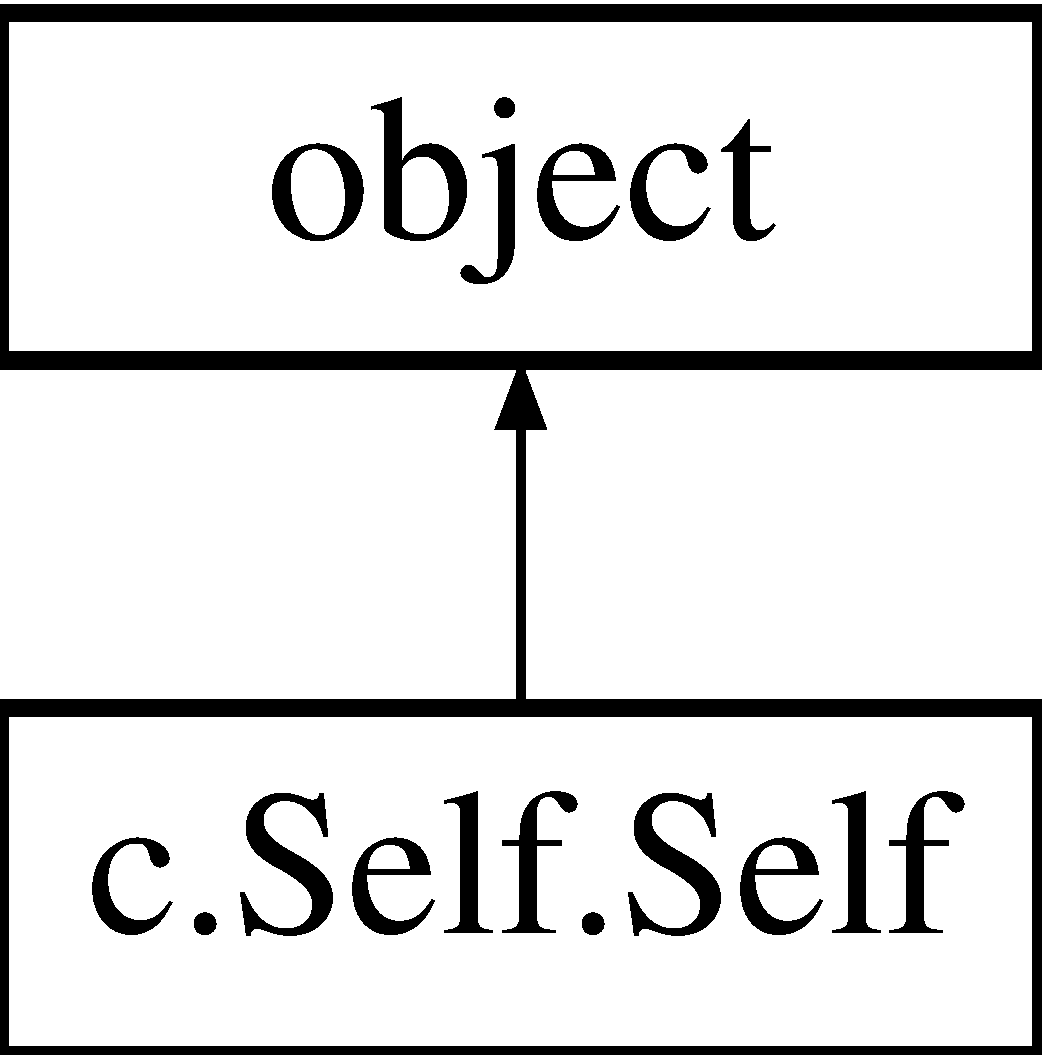
\includegraphics[height=2.000000cm]{classc_1_1_self_1_1_self}
\end{center}
\end{figure}
\subsection*{Static Public Member Functions}
\begin{DoxyCompactItemize}
\item 
def {\bfseries doc} (msg=\char`\"{}\char`\"{})\hypertarget{classc_1_1_self_1_1_self_a22c63e1abd3787d91e274dba52eefeb5}{}\label{classc_1_1_self_1_1_self_a22c63e1abd3787d91e274dba52eefeb5}

\item 
def {\bfseries name} (more=\char`\"{}\char`\"{})\hypertarget{classc_1_1_self_1_1_self_ac085532aafa2c634b302e7de5c0b67a7}{}\label{classc_1_1_self_1_1_self_ac085532aafa2c634b302e7de5c0b67a7}

\end{DoxyCompactItemize}


The documentation for this class was generated from the following file\+:\begin{DoxyCompactItemize}
\item 
Self.\+py\end{DoxyCompactItemize}

%--- End generated contents ---

% Index
\backmatter
\newpage
\phantomsection
\clearemptydoublepage
\addcontentsline{toc}{chapter}{Index}
\printindex

\end{document}
